\documentclass[addpoints]{physlabs}

\labtitle{Acceleration due to Gravity}
\labnum{}
\labnumroman{II}
\course{PHYSICS 113 - 121 - 181}
\coursesubtitle{General Physics I and Mechanics}
\date{\today}

\usetikzlibrary{patterns, angles, quotes, shapes, shapes.geometric, arrows.meta}

\begin{document}

\maketitle

% PRELAB SECTION
\begin{prelab}

    \question You have just completed the first part of this lab and have five time values for a particular height: \qty{1.8}{\second}, \qty{1.7}{\second}, \qty{1.9}{\second}, \qty{0.8}{\second}, and \qty{1.9}{\second}.
    %
    \begin{parts}
        \part[\half] Give one quantitative reason why you think that \qty{0.8}{\second} is or is not consistent with the other measurements.
        %
        \begin{solution}[1.5cm]
            
        \end{solution}

        \part[\half] If we assume that \qty{0.8}{\second} is in fact an outlier, what is one explanation for what could have gone wrong in that trial? Use details of the experiment in your answer.
        %
        \begin{solution}[1.5cm]
            
        \end{solution}
    \end{parts}

    \question[1] In this lab you will be using Atwood’s Machine to measure the acceleration due to gravity, $g$. The machine works by hanging two masses on a pulley, with each mass being acted upon by gravity. Since the masses are on opposite sides of the pulley, their weights oppose each other, and the net acceleration is less than $g$. To see this, please draw in all of the relevant forces in the diagram below. Be sure to indicate which direction friction in the pulley is acting. Assume $m_1 > m_2$.
    %
    \begin{center}
        \captionsetup{font=normalsize}
        \captionof{figure}{A cartoon of Atwood's machine. \label{fig: atwood's machine}}
        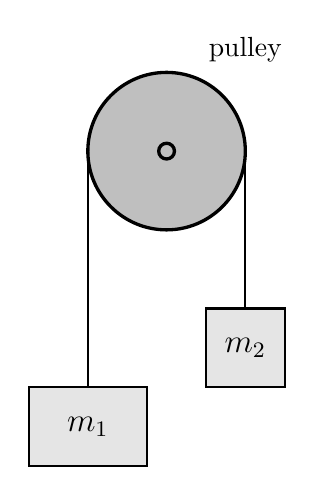
\begin{tikzpicture}
            \draw[very thick, fill=gray!50] (0,0) circle (1) node[above, yshift=10mm, xshift=10mm] {pulley};
            \draw[very thick, fill=gray!50] (0,0) circle (0.1);
            %
            \draw[thick, fill=gray!20] (-1.75,-4) rectangle (-0.25,-3) node[pos=0.5] {\large $m_1$};
            \draw[thick] (-1,-3) -- (-1,0);
            %
            \draw[thick, fill=gray!20] (0.5,-3) rectangle (1.5,-2) node[pos=0.5] {\large $m_2$};
            \draw[thick] (1,-2) -- (1,0);
        \end{tikzpicture}
    \end{center}

\end{prelab}

% LAB SECTION
\begin{labsection}

\begin{objective}
    The purpose of this lab is to demonstrate how imperfections in an experimental apparatus can play a large role in the final results. You will be measuring the acceleration of an object attached to a pulley system known as an Atwood machine (see Fig.~\ref{fig: atwood's machine}). As opposed to an object freely falling under the influence of gravity, there are other forces in an Atwood machine that slow the object down. These forces include friction in the experimental apparatus and rotational inertia, since the pulley needs to rotate for the object to fall. These extra forces mean that the acceleration of the masses is not actually given by eq.~\ref{eq: Acceleration}. In this lab, you will investigate and quantify the effects of these forces have on the acceleration of the masses.

    Additionally, you will compare two different experimental techniques to see which gives more accurate, and which gives more precise, measurements of the acceleration due to gravity, $g=\qty{9.8039}{\meter/\second^2}$. In one version of the experiment, two digital photogate timers will be used to measure how quickly the masses accelerate, and in the other, you will use hand timers. Then we will see who is better: you, or the machines. 
\end{objective}
    
\begin{theory}  
    Atwood’s machine was originally designed by George Atwood in 1784 as an experiment demonstrating the effects of uniform acceleration. 
    Atwood’s machine reduces the acceleration of the masses to a fraction of the value of gravitational acceleration, and the lower acceleration is measured to greater precision than the unchanged acceleration of gravity with the same timing device. The smaller value of the acceleration is:
    %
    \begin{equation}\label{eq: Acceleration}
        a = \frac{M_1 - M_2}{M_1 + M_2}g
    \end{equation}
    %
    Inverting this expression allows us to solve for $g$:
    %
    \begin{equation}\label{eq: Gravity}
        g = \frac{M_1 + M_2}{M_1 - M_2} a
    \end{equation}
    
    \begin{figure}[h!]
        \centering
        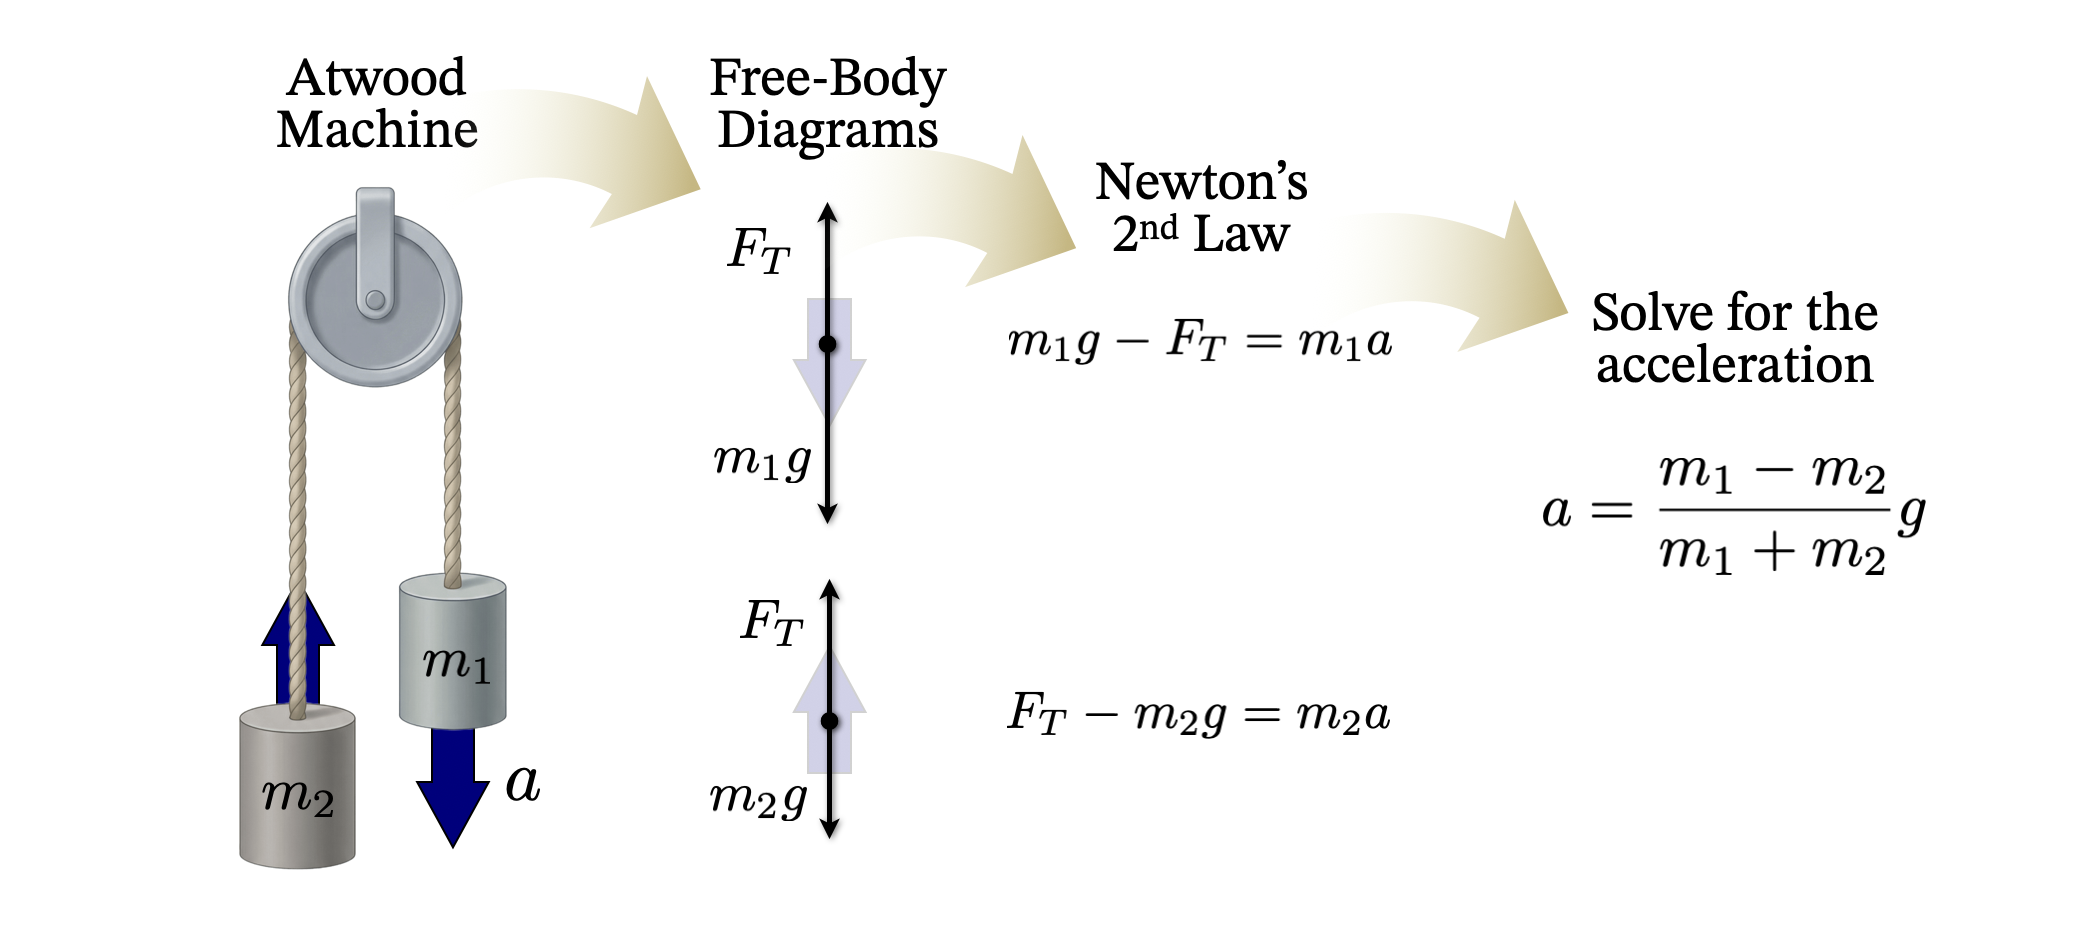
\includegraphics[width=0.85\linewidth]{AtwoodMachine.png}
        \caption{Derivation of eq.~\ref{eq: Acceleration} for Atwood's machine.}
        \label{fig: atwood's acceleration}
    \end{figure}
    
In the next section, we will show how to calculate the acceleration $a$ of the masses used in Atwood’s machine. Then, with eq.~\ref{eq: Gravity}, you will be able to estimate the acceleration due to gravity on the Earth’s surface (or at least Rochester’s surface, which is almost as good).

\subsection*{Standard Deviation of a Set of Measurements}

Throughout this lab, and in future ones, you will be asked to estimate the uncertainty in the measurements you perform. Unless are you are given further instructions, you should compute the standard deviation of a set of data, $\bar{x}_x$, using
%
\begin{align}\label{eq: Standard Deviation}
    \bar{s}^2_x &= \frac{1}{N-1}\sum_{i=1}^{N} (x_i -\bar{x})^2,
    &
    \bar{x} &= \frac{1}{N}\sum_{i=1}^N x_i,
\end{align}
%
where $x_i$ are the data points, $\bar{x}$ is the mean of the data, and $N$ is the number of data points.

For instance, if you performed 10 trials in which you timed how long it took an object to drop to the floor, measuring ten times $\{t_i\}$, you would report that the object’s fall time was the mean of your 10 data points $\bar{t}$, and the uncertainty of this fall time is the standard deviation $\bar{s}_t$. 

You could then be asked whether one of the 10 data points was consistent with others, or whether the accepted value is consistent with your findings. One way to test this is to check if the number in question lies within one (or two) standard deviation of the mean: i.e., does it lie in the range $\pm\Delta t$ or $\pm2\Delta t$. We use this test because, for a Gaussian (or normal) distribution, about 68\% of the data points should lie within one standard deviation of the mean and 95\% of the data points should lie within two standard deviations of the mean. Thus, if a number lies outside of this range, then there is a fair chance that it is an outlier.

\subsection*{The Equation of Motion for Atwood's Machine}

To find the equation of motion for the Atwood machine, we calculate the sum of the forces acting on the system. There are three force: the force of gravity on each mass $M_1$ and $M_2$, and the force due to friction in the pulley. The force due to friction is the sum of the tension in the strings on either side of the pulley $T_1$ and $T_2$ and the weight of the pulley $M_pg$ multiplied by $\mu$, the coefficient of friction.
%
\begin{equation}\label{eq: Force due to friction}
    \sum F = M_1g - M_2g - \mu(T_1 + T_2 + M_pg) = M_Ta
\end{equation}
%
Note that we have defined the direction that the larger mass $M_1$ moves to be the positive direction, $M_T$ is the total mass of the system, and $a$ is the acceleration. The total mass of Atwood's machine is made up of three separate masses: $M_1$, $M_2$, and $M_p$. Plugging in for $M_T$ on the right hand side of eq.~\ref{eq: Force due to friction} we get
%
\begin{equation}\label{eq: Force}
    M_1g - M_2g - \mu(T_1 + T_2 + M_pg) = (M_1 + M_2 + \frac{1}{2}M_p)a.
\end{equation}
%
$M_p$ is multiplied by a factor of $1/2$ because the pulley undergoing angular acceleration\footnote{This just means that the pulley is being rotated rather than pushed along a line.} rather than linear acceleration, in contrast to $M_1$ and $M_2$. The origin of the factor of $1/2$ will be covered later in the course.

\subsection*{Measuring the Acceleration $a$ with Digital Timers}

In the first part of the lab, you will measure the acceleration of the masses in the Atwood machine, $a$, and then the acceleration due to gravity, $g$, using digital timers. The mass $M_1$ will be placed in a plastic tube that will trigger the timers as it passes them. The setup is shown in Fig.~\ref{fig: atwood setup digital}.

There are four variables that must be measured to find the acceleration of gravity from this setup: $D$, the length of the plastic tube, $L$, the distance between the two photogate timers, and $t_1$ and $t_2$, the times recorded by the timers. The timers measure how long it takes an object to pass through them, so $t_1$ and $t_2$ tell us how long it takes $M_1$ to pass through the first and second timers, respectively. $M_1$ has a length of $D$, so we can find the velocity at the location of each timer by taking the distance it needed to travel and dividing by the time it took to travel that distance:

\begin{equation}\label{eq: velocity at location of timer 1}
    v_1 = \frac{D}{t_1}
\end{equation}

The speed of $M_1$ at the second timer is 
%
\begin{equation}\label{eq: velocity at location of timer 2}
    v_2 = \frac{D}{t_2}
\end{equation}

\begin{wrapfigure}[24]{l}{0.4\linewidth}
    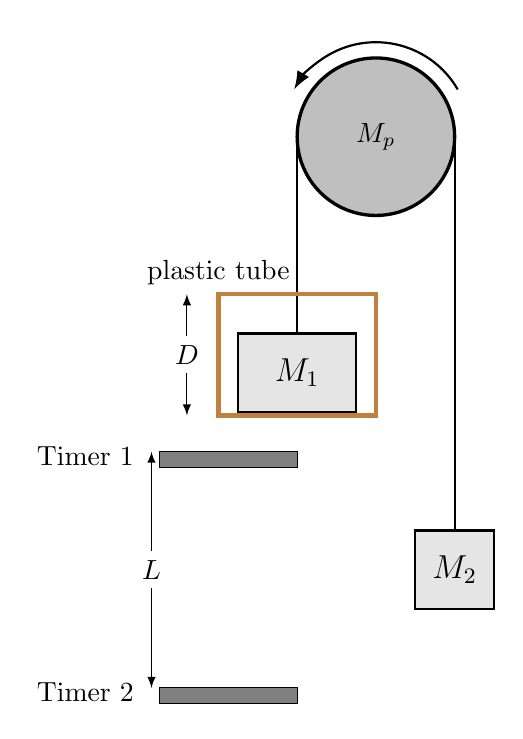
\begin{tikzpicture}
    \draw[very thick, fill=gray!50] (0,0) circle (1) node {$M_p$};
    \draw[thick, -Latex] ({1.2*cos(30)},{1.2*sin(30)}) arc (30:150:1.2);
    %
    \draw[thick, fill=gray!20] (-1.75,-3.5) rectangle (-0.25,-2.5) node[pos=0.5] {\large $M_1$};
    \draw[thick] (-1,-2.5) -- (-1,0);
    %
    \draw[ultra thick, brown] (-2,-3.54) rectangle (0,-2);
    \draw (-2,-2) node [above] {plastic tube};
    \draw[latex-latex] (-2.4,-3.54) -- node[midway,fill=white] {$D$} (-2.4,-2);
    %
    \draw[thick, fill=gray!20] (0.5,-6) rectangle (1.5,-5) node[pos=0.5] {\large $M_2$};
    \draw[thick] (1,-5) -- (1,0);
    %
    \draw[fill=gray] (-2.75,-4.2) node[left,xshift=-2mm,yshift=1.5mm] {Timer 1} rectangle (-1,-4);
    \draw[fill=gray] (-2.75,-7.2) node[left,xshift=-2mm,yshift=1.5mm] {Timer 2} rectangle (-1,-7);
    %
    \draw[latex-latex] (-2.85,-4) -- node[midway,fill=white] {$L$} (-2.85,-7);
\end{tikzpicture}
    \caption{Setup with two photogate timers.}
    \label{fig: atwood setup digital}
\end{wrapfigure}

The change in velocities is due to acceleration $a$. Using the kinematic equations, the acceleration $a$ is
%
\begin{align}\label{eq: velocity at location of timer 2}
    v_2 = v_1 + at
\end{align}
where $t$ is the time it takes $M_1$ to travel from the first timer to the second. Although the time is difficult to measure directly, the distance $L$ is easily measured. We can relate this to $t$ using another kinematic equation,
%
\begin{align}\label{eq: distance}
    L = v_1t + \frac{1}{2}at^2
\end{align}
%
From eq.~\ref{eq: velocity at location of timer 2}, we can solve for $t$ in terms of $a$:
%
\begin{align}\label{eq: time}
    t = \frac{v_2-v_1}{a}
\end{align}

Combining eqs.~\ref{eq: distance} and \ref{eq: time} to get rid of the unknown time $t$, we are left with
%
\begin{align}\label{eq: distance without t}
     \frac{v_1(v_2-v_1)}{a} + \frac{(v_2-v_1)^2}{2a} = L
\end{align}
%
Solving for the acceleration $a$ gives 
%
\begin{align}\label{eq: acceleration}
     a = \frac{D^2}{2L}\left(\frac{1}{t_2^2}-\frac{1}{t_1^2}\right).
\end{align}
%
And with that, we have found what we were looking for! By measuring a couple of lengths and using the photogate timers, we can measure how quickly the masses are accelerating. Next, we do the same for a slightly different setup.

\subsection*{Analog Hand Timer Setup}

\begin{figure}[ht]
    \centering
    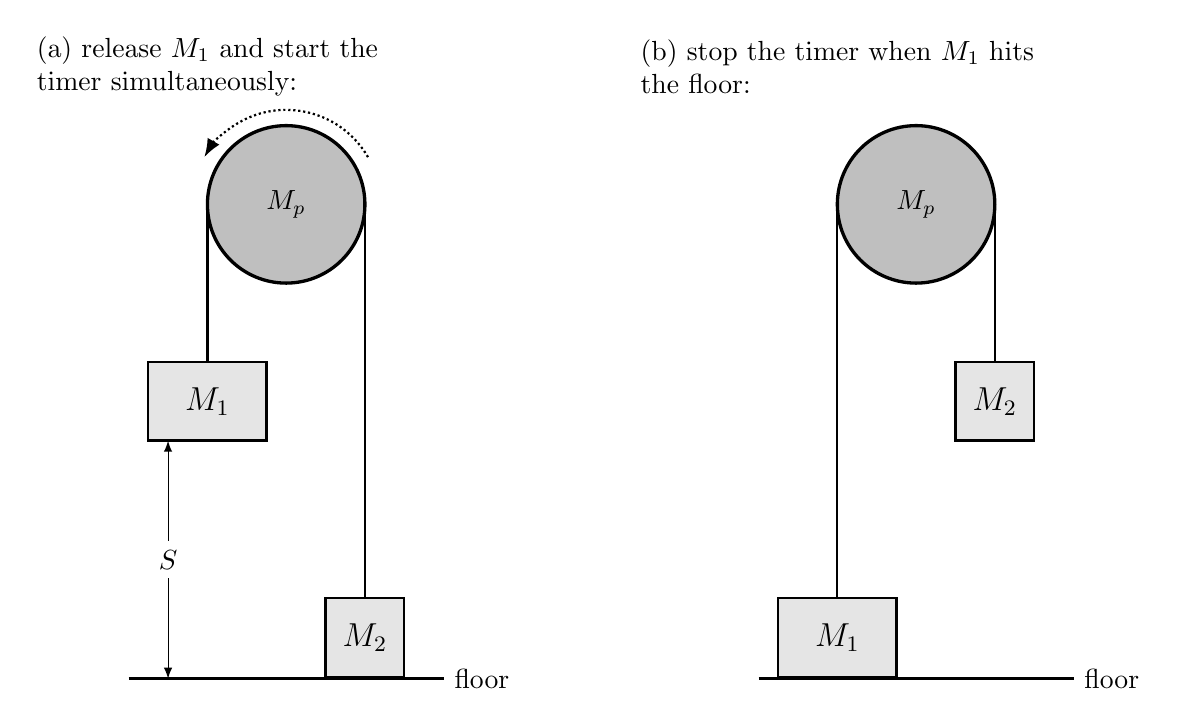
\begin{tikzpicture}
    %%% Starting position
    \draw (-1,1.75) node[align=left] {(a) release $M_1$ and start the\\timer simultaneously:};
    %
    \draw[very thick, fill=gray!50] (0,0) circle (1) node {$M_p$};
    \draw[densely dotted, thick, -Latex] ({1.2*cos(30)},{1.2*sin(30)}) arc (30:150:1.2);
    %
    \draw[thick, fill=gray!20] (-1.75,-3) rectangle (-0.25,-2) node[pos=0.5] {\large $M_1$};
    \draw[thick] (-1,-2) -- (-1,0);
    %
    \draw[thick, fill=gray!20] (0.5,-6) rectangle (1.5,-5) node[pos=0.5] {\large $M_2$};
    \draw[thick] (1,-5) -- (1,0);
    %
    \draw[very thick] (-2,-6.025) -- (2,-6.025) node[right] {floor};
    \draw[latex-latex] (-1.5,-6.025) -- node[midway,fill=white] {$S$} (-1.5,-3);
    %
    %%% Final position
    \draw ({8-1},1.75) node[align=left] {(b) stop the timer when $M_1$ hits\\the floor:};
    %
    \draw[very thick, fill=gray!50] ({0+8},0) circle (1) node {$M_p$};
    %
    \draw[thick, fill=gray!20] ({8-1.75},-6) rectangle ({8-0.25},-5) node[pos=0.5] {\large $M_1$};
    \draw[thick] ({8-1},-5) -- ({8-1},0);
    %
    \draw[thick, fill=gray!20] ({8+0.5},-3) rectangle ({8+1.5},-2) node[pos=0.5] {\large $M_2$};
    \draw[thick] ({8+1},-2) -- ({8+1},0);
    %
    \draw[very thick] ({8-2},-6.025) -- ({8+2},-6.025) node[right] {floor};
\end{tikzpicture}
    \caption{The ``analog'' setup where you manually time the fall of $M_1$. (a) Start with the setup in this position, with the lighter mass ($M_2$) on the floor. Release $M_1$ and start the timer simultaneously. (b) Stop the timer the moment $M_1$ hits the floor.}
    \label{fig: atwood setup manual}
\end{figure}

In this part of the experiment, shown schematically in Fig.~\ref{fig: atwood setup manual}, $M_1$ starts at rest, which makes the kinematics equations much simpler. Now, only two variables must be measured to find $g$, the acceleration due to gravity:
%
\begin{enumerate}
    \item The distance from the bottom of $M_1$ to the floor, denoted $S$.
    \item The time $t$ it takes for $M_1$ to reach the floor.
\end{enumerate}
%
You will measure $t$ with the hand timer.

The kinematic equations for this section are similar to those in the previous one:
%
\begin{align}
    v_\text{final} &= at & &\text{[final velocity of $M_1$]} \label{eq: atwood final velocity}
    \\
    S &= \frac{1}{2}at^2 & &\text{[distance fallen by $M_1$]} \label{eq: atwood distance}
\end{align}
%
Notice that these are eqs.~\ref{eq: velocity at location of timer 2} and \ref{eq: distance} with the initial velocity set to zero ($v_1=0$). Solving the equatios for $a$ gives
%
\begin{equation}\label{eq: acceleration simple}
    a = \frac{2S}{t^2}.
\end{equation}

The purpose of this experiment is to determine how measuring the time by hand, as George Atwood had to do in 1780s, produces different or similar measurements of $g$ compared to the use of the photogate timers.

\end{theory}
    
\begin{experiment}

\subsection*{Measuring Acceleration $a$ and $g$ using Photogates}

In this section of the lab, photogates are used to time the falling mass in Atwood's Machine. You will use the kinematic equations developed in the previous section and apply statistical techniques to produce an estimate of $g$ and its uncertainty. Before doing the experiment, \textbf{read the operating instructions on the back of the photogate}. For this experiment, you will be using the timer in gate mode. A list of equipment is given below:
%
\begin{multicols}{2}
\begin{todolist}
    \item Pulley Wheel
    \item Pole with photogates
    \item Double Pulley
    \item Photogate
    \item Photogate Timer
    \item Power cord
    \item PVC Mass Holder
    \item 3 Ring Masses
    \item Mass Holder
    \item Mass Set:
          \begin{itemize}[itemsep=0em]
              \item $1\times\qty{200}{\gram}$
              \item $2\times\qty{100}{\gram}$
              \item $1\times\phantom{0}\qty{50}{\gram}$
              \item $4\times\phantom{0}\qty{20}{\gram}$
              \item $1\times\phantom{0}\qty{10}{\gram}$
              \item $1\times\phantom{00}\qty{5}{\gram}$
          \end{itemize}
\end{todolist}
\end{multicols}

\subsubsection*{Procedure}
%
\begin{enumerate}
    \item Measure the length of the plastic tube, $D$ and the mass of the tube $M_D$. Enter your measurements in Table~\ref{tab: atwood data}.
    %
    \item Set the photogates successively along the path of the mass. Make sure that the plastic tube will not hit them on its way down.
    %
    \item Measure the distance $L$ from the top of one photogate to the top of the other photogate (see Fig.~\ref{fig: atwood setup digital}. Enter your measurement in Table~\ref{tab: atwood data}.
    %
    \item For $M_1$, add mass to the plastic tube until the total mass (including $M_D$) adds up to $M_1=\qty{260}{\gram}$. Enter the amount you added into Table~\ref{tab: atwood data}.
    %
    \item For $M_2$, add masses to one of the mass hooks until the total mass adds up to $M_2=\qty{240}{\gram}$. You may use tape to secure the masses together on the hook.
    %
    \item Once everything is set up, begin the experiment by starting the lighter mass ($M_2$) on the floor. After ensuring the photogate timers are reset, let go of the masses. Try not to push the masses when you let them go; you will only be able to measure the acceleration due to gravity if they start from rest. Hold the pulley and not the masses to keep them steady for the fall.
    %
    \item Record the time from the top timer as $t_1$, and the time from the bottom timer as $t_2$, in Table~\ref{tab: photogate data}. Note that $t_1$ is the time the photogate initially displays. After you have recorded $t_1$, find $t_2$ by flipping the \texttt{MEMORY} switch on the photogate to \texttt{READ}. The new number displayed will be $t_1+t_2$; subtract $t_1$ from this value to get $t_2$ and record it. To confirm that your numbers are reasonable, check that $t_2>t_1$.
    %
    \item Repeat the measurement 10 times to get a good estimate of the average value of $g$ and its standard deviation, which we will use for our uncertainty. Enter all values in Table~\ref{tab: photogate data}.
\end{enumerate}

\begin{table}[ht]
    \centering
    \renewcommand{\arraystretch}{2.2}
    \captionsetup{font=normalsize}
    \caption{Lengths and masses used in the Atwood machine. In column 4, indicate the amount of mass you added to the tube to get $M_1$ to \qty{260}{\gram}. \label{tab: atwood data}}
    \begin{tabular}{|>{\centering\arraybackslash}p{1.6cm}|>{\centering\arraybackslash}p{1.6cm}|>{\centering\arraybackslash}p{1.6cm}|>{\centering\arraybackslash}p{1.6cm}|>{\centering\arraybackslash}p{1.6cm}|>{\centering\arraybackslash}p{1.6cm}|}
    \hline
    \rowcolor{gray!20}
    $D$ [cm] & $L$ [cm] & $M_D$ [g] & $M_1-M_D$ [g] & $M_1$ [g] & $M_2$ [g] \\
    \hline
             &          &           &               & 260       & 240       \\
    \hline
    \end{tabular}
\end{table}

\begin{table}[ht]
    \centering
    \renewcommand{\arraystretch}{2.2}
    \captionsetup{font=normalsize}
    \caption{Atwood machine $M_1$ fall times using photogates. \label{tab: photogate data}}
    \begin{tabular}{|c|>{\centering\arraybackslash}p{2cm}|>{\centering\arraybackslash}p{2cm}|c|>{\centering\arraybackslash}p{2cm}|>{\centering\arraybackslash}p{2cm}|}
    \hline
    \rowcolor{gray!20}
    Trial & $t_1$ [sec] & $t_2$ [sec] & Trial & $t_1$ [sec] & $t_2$ [sec] \\
    \hline
    1     &             &             & 6     &             &             \\
    \hline
    2     &             &             & 7     &             &             \\
    \hline
    3     &             &             & 8     &             &             \\
    \hline
    4     &             &             & 9     &             &             \\
    \hline
    5     &             &             & 10    &             &             \\
    \hline
    \end{tabular}
\end{table}

\subsection*{Measuring Acceleration $a$ and $g$ with Manual Timers}

This setup is the same as your previous measurement, minus the photogate timers. Move the photogates out of the way to ensure that the mass doesn’t knock into them while it is falling.

\subsubsection*{Procedure}

\begin{enumerate}
    \item Let $M_1$ (the plastic tube) lie on the floor and measure the distance, $S$, from the floor to the bottom of the lighter mass ($M_2$). Do not hold the masses or the string when measuring; otherwise, you will not get an accurate measurement.
    %
    \item Familiarize yourself with the hand timer and plug it in when you are ready to use it. If you prefer, you may also use a phone or any other device that can be used as a stopwatch.
    %
    \item The experiment is the same as before. Hold $M_2$ on the floor and then release it, and time how long it takes $M_1$ to reach the floor.
    %
    \item Use your chosen timing device and make 10 measurements of how long it
takes $M_1$ to travel the distance $S$. Make sure you release the masses and start the timer simultaneously. Record the times in Table~\ref{tab: timer data}. 
\end{enumerate}

\begin{table}[ht]
    \centering
    \renewcommand{\arraystretch}{2.2}
    \captionsetup{font=normalsize}
    \caption{Atwood machine $M_1$ fall times using manual timers. \label{tab: timer data}}
    \begin{tabular}{|c|>{\centering\arraybackslash}p{2cm}|>{\centering\arraybackslash}p{2cm}|c|>{\centering\arraybackslash}p{2cm}|>{\centering\arraybackslash}p{2cm}|}
    \hline
    \rowcolor{gray!20}
    Trial & $t_1$ [sec] & $t_2$ [sec] & Trial & $t_1$ [sec] & $t_2$ [sec] \\
    \hline
    1     &             &             & 6     &             &             \\
    \hline
    2     &             &             & 7     &             &             \\
    \hline
    3     &             &             & 8     &             &             \\
    \hline
    4     &             &             & 9     &             &             \\
    \hline
    5     &             &             & 10    &             &             \\
    \hline
    \end{tabular}
\end{table}

\subsection*{Accounting for the Rotational Inertia of the Pulley}

When you try to move an object in a straight line, it is clear that the higher the mass of the object, the harder you have to push to get the same acceleration. A similar rule applies to spinning objects. A car wheel is harder to spin than a bicycle wheel because the car wheel is much heavier.

Spinning objects are more complicated because their motion depends not only on their mass, but also on how the mass is distributed around the axis of rotation. You will deal with this complication formally later in the course. For now, we will confine ourselves to relatively simple objects.

In the previous measurements and in the corresponding sections of the Postlab exercises, we treat the acceleration of the masses as if the pulley is massless. However, the pulley does have mass and is accelerated as the masses fall. Does the extra force required to spin the pulley affect the experiment? In this section, you will carry out measurements that account for the mass of the pulley, and in the final section of the Postlab exercises, you will determine the effect of the pulley’s mass on your measurement of $g$ (if any).

\subsubsection*{Procedure}

\begin{enumerate}
    \item Replace the current pulley system with the large-disk pulley.
    %
    \item Attach two metal mass holders to the pulley and add masses to the holders so that they match the first combination of $M_1$ and $M_2$ given in Table~\ref{tab: pulley data} below.
    %
    \item As in the second part of the lab, measure the distance, $S$, from the floor to the bottom of the lighter mass $M_2$ while the heavier mass $M_1$ sits on the floor. Fill in the result below in Table~\ref{tab: pulley data}.
    %
    \item For each combination of $M_1$ and $M_2$ listed in Table~\ref{tab: pulley data}, measure the drop time once using the hand timers. Record these values in column ``$M_\text{ring}=0$'' in the table.
    %
    \item Measure the mass of one of the metal rings ($M_\text{ring}$) and add this to the pulley. Record $M_\text{ring}$ in Table~\ref{tab: pulley data} and repeat the previous step: for each combination of $M_1$ and $M_2$, measure the drop time once using the hand timers and record these values in the middle column of Table~\ref{tab: pulley data}.
    %
    Measure the mass of a second metal ring and add this to the pulley as well. Record $2M_\text{ring}$ in Table~\ref{tab: pulley data} and repeat the previous steps: for each combination of $M_1$ and $M_2$, measure the drop time once using the hand timers and record these values in the right column of Table~\ref{tab: pulley data}.
\end{enumerate}

\begin{table}[ht]
    \centering
    \renewcommand{\arraystretch}{2.2}
    \captionsetup{font=normalsize}
    \caption{Manual timing data with the large pulley and ring masses. \label{tab: pulley data}}
    \begin{tabular}{|>{\centering\arraybackslash}p{1cm}|>{\centering\arraybackslash}p{1cm}|>{\centering\arraybackslash}p{3.5cm}|>{\centering\arraybackslash}p{3.5cm}|>{\centering\arraybackslash}p{3.5cm}|}
    \hline
    \multirow{2}{*}{$M_1$} & \multirow{2}{*}{$M_2$} & \multicolumn{3}{c|}{Fall times [s]}                                           \\
    \cline{3-5}
                           &                        & $M_\text{ring}=0$ & $M_\text{ring}=\uline{\qquad\qquad}$ [g] & $2M_\text{ring}=\uline{\qquad\qquad}$ [g] \\
    \hline
    \qty{105}{\gram}       & \qty{100}{\gram}       &                   &                            &                             \\
    \hline
    \qty{110}{\gram}       & \qty{100}{\gram}       &                   &                            &                             \\
    \hline
    \qty{115}{\gram}       & \qty{100}{\gram}       &                   &                            &                             \\
    \hline
    \end{tabular}
\end{table}

\end{experiment}

\end{labsection}

\begin{postlab}

    %%% First part: measurement with photogates
    \fullwidth{\subsection*{Measurement using Photogate Timers (\pointsinrange{photogate} points)}}

    \begingradingrange{photogate}
    
    \filbreak
    \question[1] Calculate averages of your time data, $\bar{t}_1$ and $\bar{t}_2$, as well as the standard deviations $\Delta t_1$ and $\Delta t_2$, using your measurements from Table~\ref{tab: photogate data}. Remember to include units!

    {\renewcommand{\arraystretch}{2.2}
    \begin{tabular}{lp{3cm}}
        $\bar{t}_1=$  &  \\
        \cline{2-2}
        $\bar{t}_2=$  &  \\
        \cline{2-2}
        $\Delta t_1=$ &  \\
        \cline{2-2}
        $\Delta t_2=$ &  \\
        \cline{2-2}
    \end{tabular}}
    
    \begin{solution}[1cm]
        
    \end{solution}

    \filbreak
    \question[1] Find the average acceleration using eq.~\ref{eq: acceleration}. For $t_1$ and $t_2$, plug in the average values $\bar{t}_1$ and $\bar{t}_2$ you just computed. Show all work and express your result in correct units.

    {\renewcommand{\arraystretch}{2.2}
    \begin{tabular}{lp{3cm}}
        $\bar{a}=$  &  \\
        \cline{2-2}
    \end{tabular}}

    \begin{solution}[1cm]
        
    \end{solution}

    \filbreak
    \question
    \begin{parts}
        \part[1] Base your uncertainties in $L$ ($\Delta L$) and $D$ ($\Delta D$) on how accurately you think you read the ruler. Use the error propagation formula below to estimate $\Delta a$, the uncertainty on the acceleration:
        \[
            \Delta a = \bar{a}\cdot\sqrt{\left(\frac{\Delta L}{L}\right)^2 + \left(\frac{2\Delta D}{D}\right)^2 + \left(\frac{2\Delta t_1}{\bar{t}_1}\right)^2 + \left(\frac{2\Delta t_2}{\bar{t}_2}\right)^2}.
        \]
        Include units with your values.

        {\renewcommand{\arraystretch}{2.2}
        \begin{tabular}{lp{3cm}}
            $\Delta L=$  &  \\
            \cline{2-2}
            $\Delta D=$  &  \\
            \cline{2-2}
            $\Delta a=$  &  \\
            \cline{2-2}
        \end{tabular}}
        
        \begin{solution}[0.5cm]
        \end{solution}

        \part[\half] Which of the four terms in the square root of the error propagation equation above contributed the most to the uncertainty $\Delta a$?
        \begin{solution}[1.5cm]
        \end{solution}

        \part[\half] What is one possible reason that this term added the most uncertainty?
        \begin{solution}[1.5cm]
        \end{solution}
    \end{parts}

    \endgradingrange{photogate}

    %%% Second part: measurement with hand timers
    \fullwidth{\subsection*{Measurement using Manual Timers (\pointsinrange{manual} points)}}

    \begingradingrange{manual}

    \filbreak
    \question[1] Calculate the mean and standard deviation of your hand timer data (Table~\ref{tab: timer data}). Include units with your values.

    {\renewcommand{\arraystretch}{2.2}
    \begin{tabular}{lp{3cm}}
        $\bar{t}=$  &  \\
        \cline{2-2}
        $\Delta t=$  &  \\
        \cline{2-2}
    \end{tabular}}
    
    \begin{solution}[0.5cm]
    \end{solution}

    \filbreak
    \question[1] Find the average acceleration using eq.~\ref{eq: acceleration simple}. For $t$, plug in the average value $\bar{t}$ you just computed. Show all work and express your result in correct units.

    {\renewcommand{\arraystretch}{2.2}
    \begin{tabular}{lp{3cm}}
        $\bar{a}=$  &  \\
        \cline{2-2}
    \end{tabular}}

    \begin{solution}[1cm]
        
    \end{solution}

    \filbreak
    \question
    \begin{parts}
        \part[1] Base your uncertainties in $S$ ($\Delta S$) on how accurately you think you read the ruler. Use the error propagation formula below to estimate $\Delta a$, the uncertainty on the acceleration:
        \[
            \Delta a = \bar{a}\cdot\sqrt{\left(\frac{\Delta S}{S}\right)^2 + \left(\frac{2\Delta t_2}{\bar{t}_2}\right)^2}.
        \]
        Include units with your values.

        {\renewcommand{\arraystretch}{2.2}
        \begin{tabular}{lp{3cm}}
            $\Delta S=$  &  \\
            \cline{2-2}
            $\Delta a=$  &  \\
            \cline{2-2}
        \end{tabular}}
        
        \begin{solution}[0.5cm]
        \end{solution}

        \part[1] Which quantity, $S$ or $t$, contributes the most to our uncertainty $\Delta a$ in the estimate of the acceleration $\bar{a}$?
        \begin{solution}[1.5cm]
        \end{solution}
    \end{parts}

    \filbreak
    \question[1] \label{q: g results} Use eq.~\ref{eq: Gravity} to estimate $g$ from the photogate and manual timer data. Also, compute the uncertainty on $g$ using the error propagation formula
    \[
        \Delta g = \frac{M_1+M_2}{M_1-M_2}\Delta a.
    \]
    Include units with your values.

    {\renewcommand{\arraystretch}{2.2}
    \begin{tabular}{lp{3cm}cp{3cm}}
        $g_\text{photogate}=$  & & $\pm$ & \\
        \cline{2-2}\cline{4-4}
        $g_\text{hand timer}=$ & & $\pm$ & \\
        \cline{2-2}\cline{4-4}
    \end{tabular}}

    \begin{solution}[1cm]
    \end{solution}

    \filbreak
    \question Compare the accuracy and precision of the two results, one using the hand timer and the other using the photogate timers. Remember the accepted value of $g=\qty{9.8039}{\meter/\second^2}$.
    %
    \begin{parts}
        \part[1] Which method was more precise? Explain why based on your estimates for $g$.
        \begin{solution}[2cm]
            The result with the smaller standard deviation is more precise. The likely answer is the photogate.
        \end{solution}

        \part[1] Which method was more accurate? Explain why based on your estimates for $g$.
        \begin{solution}[2cm]
            The result closer to the accepted value is more accurate. The likely answer is the photogate.
        \end{solution}

        \part[1] How many standard deviations, $N_\text{SD}$, are your two estimates for $g$ from each other? Use the formula below to compute your answer:
        \[
            N_\text{SD} = \left|\frac{g_\text{photogate}-g_\text{hand timer}}{\Delta g_\text{photogate}+\Delta g_\text{hand timer}}\right|.
        \]
        \begin{solution}[2cm]
            Students should compute and report their results.
        \end{solution}
        
    \end{parts}

    \endgradingrange{manual}

    %%% Third part: corrections for the mass of the pulley
    \fullwidth{\subsection*{Accounting for the Rotational Inertia of the Pulley (\pointsinrange{pulley} points)}}

    \begingradingrange{pulley}

    \filbreak
    \question[1] Using the data you recorded in Table~\ref{tab: pulley data}, calculate $(M_1-M_2)/(M_1+M_2)$ for each combination of $M_1$ and $M_2$ used in the measurement. Then compute the acceleration for each trial using eq.~\ref{eq: acceleration simple}. Don't forget to include units!

    \begin{center}
        \renewcommand{\arraystretch}{2.2}
        \captionsetup{font=normalsize}
        \captionof{table}{Estimated acceleration with the large pulley and ring masses. \label{tab: pulley acceleration}}
        \begin{tabular}{|>{\centering\arraybackslash}p{2cm}|>{\centering\arraybackslash}p{3.5cm}|>{\centering\arraybackslash}p{3.5cm}|>{\centering\arraybackslash}p{3.5cm}|}
        \hline
    \multirow{2}{*}{$\displaystyle\frac{M_1-M_2}{M_1+M_2}$} & \multicolumn{3}{c|}{Acceleration} \\
        \cline{2-4}
                                               & 0 rings   & 1 ring   & 2 rings   \\
        \hline
                                               &           &          &           \\
        \hline
                                               &           &          &           \\
        \hline
                                               &           &          &           \\
        \hline
        \end{tabular}
    \end{center}

    \filbreak
    \question[2] If the pulley is massless, then eq.~\ref{eq: Acceleration} holds and 
    \[
        a = \frac{M_1-M_2}{M_1+M_2} g.
    \]
    Thus, a plot of $a$ versus $(M_1-M_2)/(M_1+M_2)$ should result in a straight line with a slope of $g$. To see if the mass of the pulley affects our data, we can make such a plot and compare the slope to the accepted value $g=\qty{9.8039}{\meter\second^2}$.

    Plot $a$ versus the mass ratio $(M_1-M_2)/(M_1+M_2)$ on the grid below for the 0-ring data and draw a best-fit straight line through your points. Then do the same for the 1-ring and the 2-ring data. Make sure to include axis labels, units, and titles for your plot. Add a legend or otherwise indicate which points belong to the 0-ring, 1-ring, and 2-ring measurements.\\[0em]

    \begin{center}
        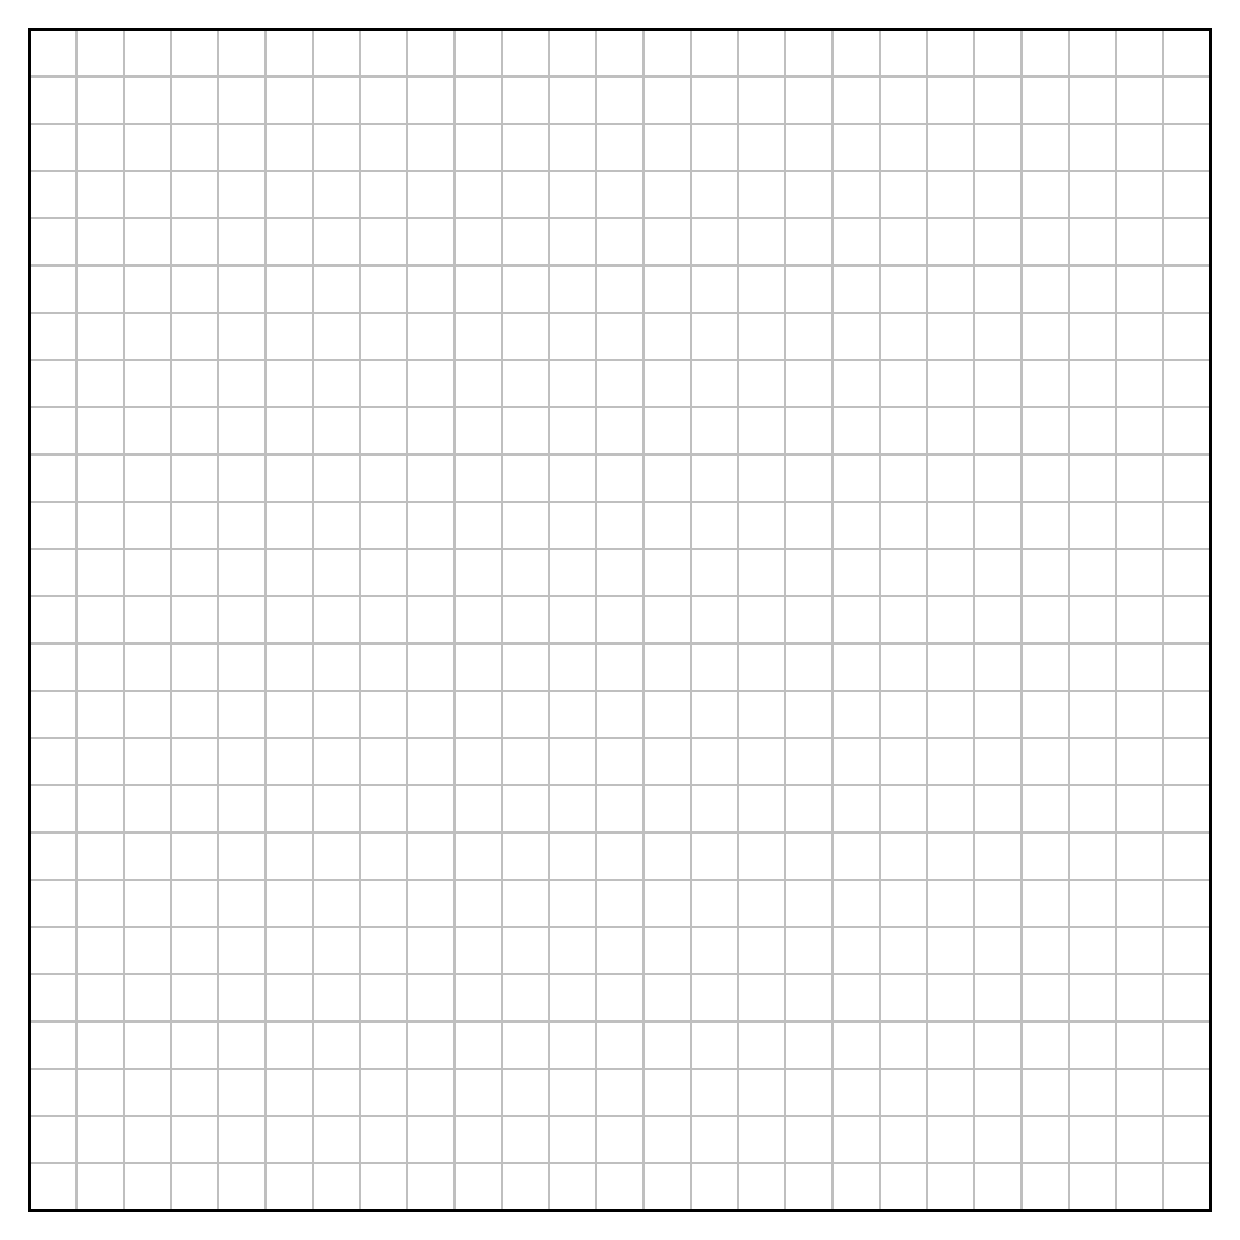
\begin{tikzpicture}
            % Define dimensions
            \def\gridwidth{25}
            \def\gridheight{25}
            \def\spacing{0.6}
            % Draw grid paper on the left
            \begin{scope}[xshift=0cm,yshift=0cm]
                % Major grid lines (thicker)
                \foreach \x in {0,1,...,\gridwidth}
                    \draw[gray!50,thick] (\x*\spacing,0) -- (\x*\spacing,\gridheight*\spacing);
                \foreach \y in {0,1,...,\gridheight}
                    \draw[gray!50, thick] (0,\y*\spacing) -- (\gridwidth*\spacing,\y*\spacing);
                \draw[black, very thick] (0,0) rectangle (\gridwidth*\spacing,\gridheight*\spacing);
            \end{scope}
        \end{tikzpicture}
    \end{center}

    \filbreak
    \question[1] \label{q: slope g} How does your measurement for $g$ change as the mass of the pulley increases? \textsl{Hint: remember that $g$ should be equal to the slope of your data.}
    %
    \begin{solution}[3cm]
        
    \end{solution}

    \filbreak
    \question[1] Given your answer to question~\ref{q: slope g}, do you think the effect of the pulley's mass on measurements of $g$ can be used to explain the differences between your estimates for $g$ in question~\ref{q: g results}, and the accepted value of $g=\qty{9.8039}{\meter\second^2}$?
    %
    \begin{solution}[2cm]
        
    \end{solution}

    \filbreak
    \question[1] What is another significant source of error in Atwood's machine that is not explored in this lab? How might this affect your results?
    %
    \begin{solution}[2cm]
        
    \end{solution}

    \filbreak
    \question
    \begin{parts}
        \part[\half] What is one improvement you could make to Atwood's machine to improve the accuracy of your results?
        \begin{solution}[1.5cm]
            
        \end{solution}

        \part[\half] What is one improvement that would make the results more precise?
        \begin{solution}[1.5cm]
            
        \end{solution}
    \end{parts}

    \filbreak
    \question[1] Clearly, Atwood's machine has a lot of systematic errors that would not be present if we were to simplify the experiment. What is one reason we might expect to get better results using Atwood's machine rather than following Galileo’s example and just dropping objects off of tall buildings?
    %
    \begin{solution}[1.5cm]
            
    \end{solution}

    \endgradingrange{pulley}
    
\end{postlab}

\end{document}